\documentclass[10pt,twocolumn,letterpaper]{article}

% Pacotes basicos - maxima compatibilidade Windows
\usepackage{geometry}
\usepackage{times}
\usepackage{titlesec}
\usepackage{url}
\usepackage{graphicx,xcolor,comment,enumerate,multirow,multicol, float} 
\usepackage{amsmath,amsthm,amsfonts,amssymb,dsfont,mathtools,array}

\renewcommand{\tablename}{Tabela}

% \input{cor.tex}

% Configuracao da pagina
\geometry{
    letterpaper,
    left=0.75in,
    right=0.75in,
    top=0.75in,
    bottom=1in
}

% Configuracao das secoes
\titleformat{\section}[block]
{\normalfont\fontsize{10}{12}\bfseries}
{\thesection.}{0.5em}{}

% Remove numeracao das paginas
\pagestyle{empty}

% Configuracoes de espacamento
\setlength{\columnsep}{0.25in}
\setlength{\parindent}{0pt}
\setlength{\parskip}{6pt}

\begin{document}

% Titulo centralizado em coluna unica
\twocolumn[
\begin{center}
    {\fontsize{16}{19}\selectfont\bfseries 
    Experimento 3\\ Estudo dirigido sobre estruturas cristalinas}

    \vspace{1cm}
    
    {\fontsize{11}{13}\selectfont 
     Larissa Simões – 232028230, Carlos Eduardo da S. Papa – 232013390, Thiago Ferreira – 232028230}

    \vspace{0.35cm}   

    {\fontsize{11}{13}\selectfont 
    Turma 01}
    
    \vspace{1cm}  
\end{center}
]

\section{OBJETIVOS}

\hspace{1cm} Este experimento tem como objetivo analisar a resposta em corrente contínua (DC) de um sensor de efeito Hall fabricado pela Honeywell, caracterizando seu comportamento frente a variações do campo magnético aplicado. Busca-se, a partir dessa análise, estimar o valor do campo magnético B
 gerado no circuito magnético e, posteriormente, determinar a permeabilidade magnética efetiva da ferrite utilizada no núcleo do sensor.

% \begin{figure}[h]
%     \centering
%     
\includegraphics[width=5cm]{PrimitiveCell.png}
%     \caption{EXEMPLO DE IMAGEM}
%     \label{fig:label}
% \end{figure}

% \vspace{.75cm}

\section{MATERIAIS e EQUIPAMENTO UTILIZADOS}

\begin{itemize}
    \item Sensor Hall de Corrente (Honeywell – CSLA1CD) com
regulador de tensão;
    \item Ponte de Impeâncias 1650-A ou 1650-B da General
    Radio;
    \item Varivolt (0-240 Vac) com cabo para adaptação à tomada;
    \item Fonte LEEPUC Mod.402-A (2);
    \item Multímetro (2);
    \item Resistor limitador de corrente;
    \item Cabos banana e garras.
\end{itemize}

% \vspace{.75cm}

\section{PROCEDIMENTOS EXPERIMENTAIS}

\noindent\textit{Parte 1: medição da tensão de saída do sensor hall:}

\hspace{1cm}   Essa etapa tem como finalidade levantar a curva característica de resposta do sensor, para verificar sua sensibilidade à corrente aplicada e à densidade de fluxo magnético induzida. Inicialmente, nosso grupo montou o arranjo experimental conforme o diagrama de circuito mostrado na Figura 1 assegurando posicionamento correto do sensor no interior do circuito magnético e a conexão dos instrumentos de medição.
Com o circuito já ajustado, foi feita a variação gradual da corrente contínua (DC) aplicada ao enrolamento, e  registramos os valores correspondentes da tensão de saída do sensor Hall.  A partir desses dados, foi possível observar a relação linear entre a tensão Hall e o campo magnético gerado, confirmando a proporcionalidade esperada entre 
Vh e B.

\begin{equation*}
    V_H = \frac{R_H I B}{t} 
\end{equation*}

\noindent\textit{Parte 2: Determinação da permeabilidade e relutância do circuito magnético}

\hspace{1cm} Na segunda etapa caracterizamos as propriedades magnéticas do núcleo de ferrite utilizado no sensor. Para isso, medimos a indutância do enrolamento associado ao circuito magnético conectando os terminais do enrolamento a uma ponte de impedâncias. O instrumento foi ajustado até o equilíbrio, e registramos o valor da indutância "L" e o correspondente fator de qualidade (Q). Sabe-se que a indutância de uma bobina é diretamente proporcional à permeabilidade magnética do meio e inversamente proporcional à relutância do circuito, de modo que:

\begin{equation*}
    L = \frac{N^2}{\mathfrak{R}}
\end{equation*}

onde "N" é o número de espiras e 
"R" é a relutância magnética total. Assim, conhecendo "L"
é possível estimar a densidade de fluxo magnético "B"
gerada para diferentes valores de corrente no enrolamento.


\hspace{1cm} Com esses resultados foi possível correlacionar a tensão de saída do sensor Hall com o campo magnético efetivo produzido pelo circuito, determinando experimentalmente a sensibilidade do sensor e analisando o comportamento do material de ferrite variando corrente e do campo aplicado.

% \vspace{-.25cm}

\begin{figure}[h]
    \centering
    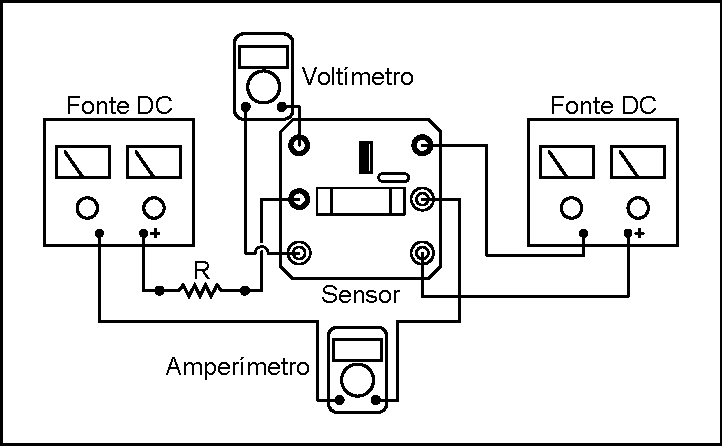
\includegraphics[width=8cm]{Ativo 1.pdf}
    \caption{Diagrma do circuito implementado}
    \label{fig:circuito_implementado}
    \vspace{-.25cm}
\end{figure}

% \vspace{.25cm}

\section{RESULTADOS EXPERIMENTAIS}

\hspace{1cm} Seguindo o procedimento proposto para a primeira etapa, foram determinados os valores de indutância e fator de qualidade (Q) do enrolamento, conforme Tabela I.

% \vspace{-.35cm}

\begin{table}[h]
    \centering
    \caption{Indutância e fator de qualidade medido}
    \label{tab:your_table_label}
    \vspace{0.25cm}
    \begin{tabular}{ >{\centering\arraybackslash}m{3cm}  >{\centering\arraybackslash}m{3cm} }
        \hline
        \textbf{Indutância [$\mu H$]} & \textbf{Fator de qualidade} \\
        \hline
        L = 128 & Q = 2.6 \\
        \hline
    \end{tabular}
\end{table}

% \vspace{-.25cm}

\begin{figure}[h]
    \centering
    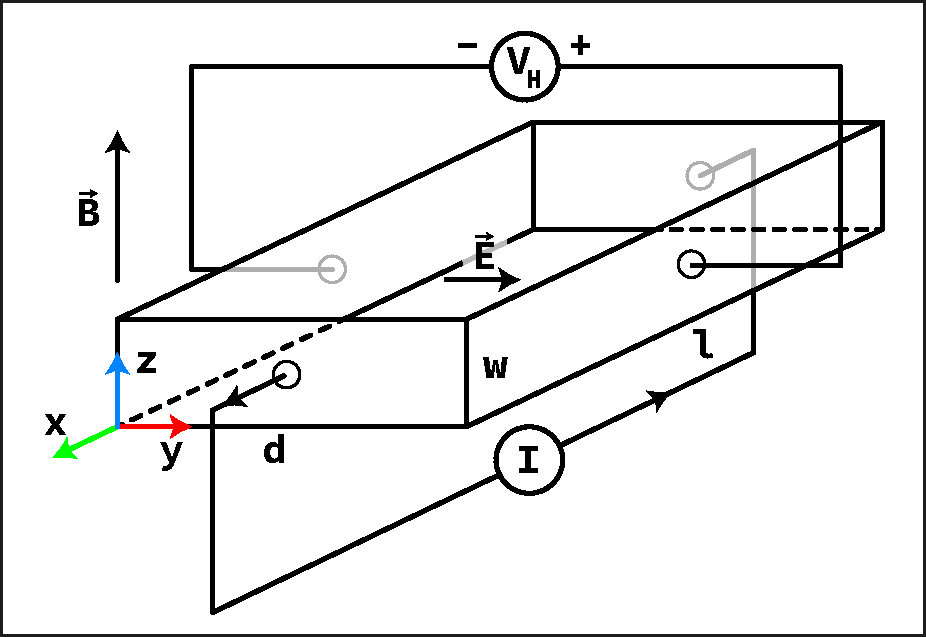
\includegraphics[width=7.25cm]{Ativo 2.pdf}
    \caption{Diagrma dos campos}
    % \vspace{-.25cm}
    \label{fig:campos}
\end{figure}

\hspace{1cm} Em continuidade, na segunda etapa, foram obtidos os valores de corrente contínua (DC) e das respectivas tensões de saída, apresentados na Tabela II. Observa-se que, diferentemente do que ocorre em representações ideais, o sensor de corrente Honeywell – CSLA1CD apresenta um valor de tensão de offset distinto de zero mesmo para corrente nula (0 A), devido à forma como a medição é realizada em diferentes pontos do eixo $x$. Por essa razão, a segunda coluna da tabela foi normalizada, de modo a compensar o valor de offset e permitir uma análise comparativa mais coerente entre as medições.

\begin{table}[htbp]
    \centering
    \caption{Medições de Tensão em Função da Corrente DC}
    \label{tab:medicoes_tensao}
    \vspace{0.25cm}
    \begin{tabular}{ccc}
        \hline
        \rule{0pt}{3ex}\textbf{Corrente DC [A]} & \textbf{V}$_{saida}$ \textbf{s/ offset [V]} & \textbf{V [V]} \\ [5pt]
        \hline
        \rule{0pt}{3ex}1.4   & 3.22 &  9.63 \\
        1.2   & 2.81 &  9.22 \\
        1     & 2.39 &  8.80 \\
        0.8   & 1.94 &  8.35 \\
        0.6   & 1.47 &  7.88 \\
        0.4   & 0.97 &  7.38 \\
        0.2   & 0.50 &  6.91 \\
        0     & 0.00 &  6.41 \\
        -0.2  & -0.49 &  5.92 \\
        -0.4  & -1.00 &  5.41 \\
        -0.6  & -1.46 &  4.95 \\
        -0.8  & -1.95 &  4.46 \\
        -1.0  & -2.41 &  4.00 \\
        -1.2  & -2.84 &  3.57 \\
        -1.4  & -3.27 &  3.14 \\ [5pt]
        \hline
    \end{tabular}
\end{table}

% \vspace{.75cm}

\section{ANALISE DOS RESULTADOS EXPERIMENTAIS}

\hspace{1cm} Com base nos valores medidos de indutância e nas dimensões geométricas do circuito magnético $(l_g, l_f \,\text{e} \, A)$, foi possível calcular a permeabilidade da ferrite e a relutância total do sistema, utilizando as equações apresentadas a seguir:
% \vspace{-.25cm}
\begin{equation*}
    L = \frac{N^2}{\mathfrak{R}}
\end{equation*}
% \vspace{-.25cm}
\begin{equation*}
    \mathfrak{R} = \frac{l_g}{\mu_0A} + \frac{l_f}{\mu_fA}
\end{equation*}

\hspace{1cm} Considerando que o enrolamento contém N=50 espiras, a relutância total foi obtida pela expressão:

\begin{equation*}
    \mathfrak{R} = \frac{50^2}{170\cdot10^{-6}} = 14705882.352941 \, \left[\frac{Ae}{Wb}\right]
\end{equation*}

\hspace{1cm} Com esses dados, determinou-se a permeabilidade magnética efetiva do material:

\begin{equation*}
    \mu_f = \left[ \left( \mathfrak{R} - \frac{l_g}{\mu_0A} \right) \frac{A}{l_f} \right]^{-1} = -4.16207 \cdot 10^{-5} \, \left[\frac{H}{m}\right]
\end{equation*}

\hspace{1cm} Após a coleta completa dos dados e o preenchimento da Tabela II, foi construída a curva da tensão de saída em função da corrente, ilustrada na Figura 3.

\begin{figure}[h]
    \centering
    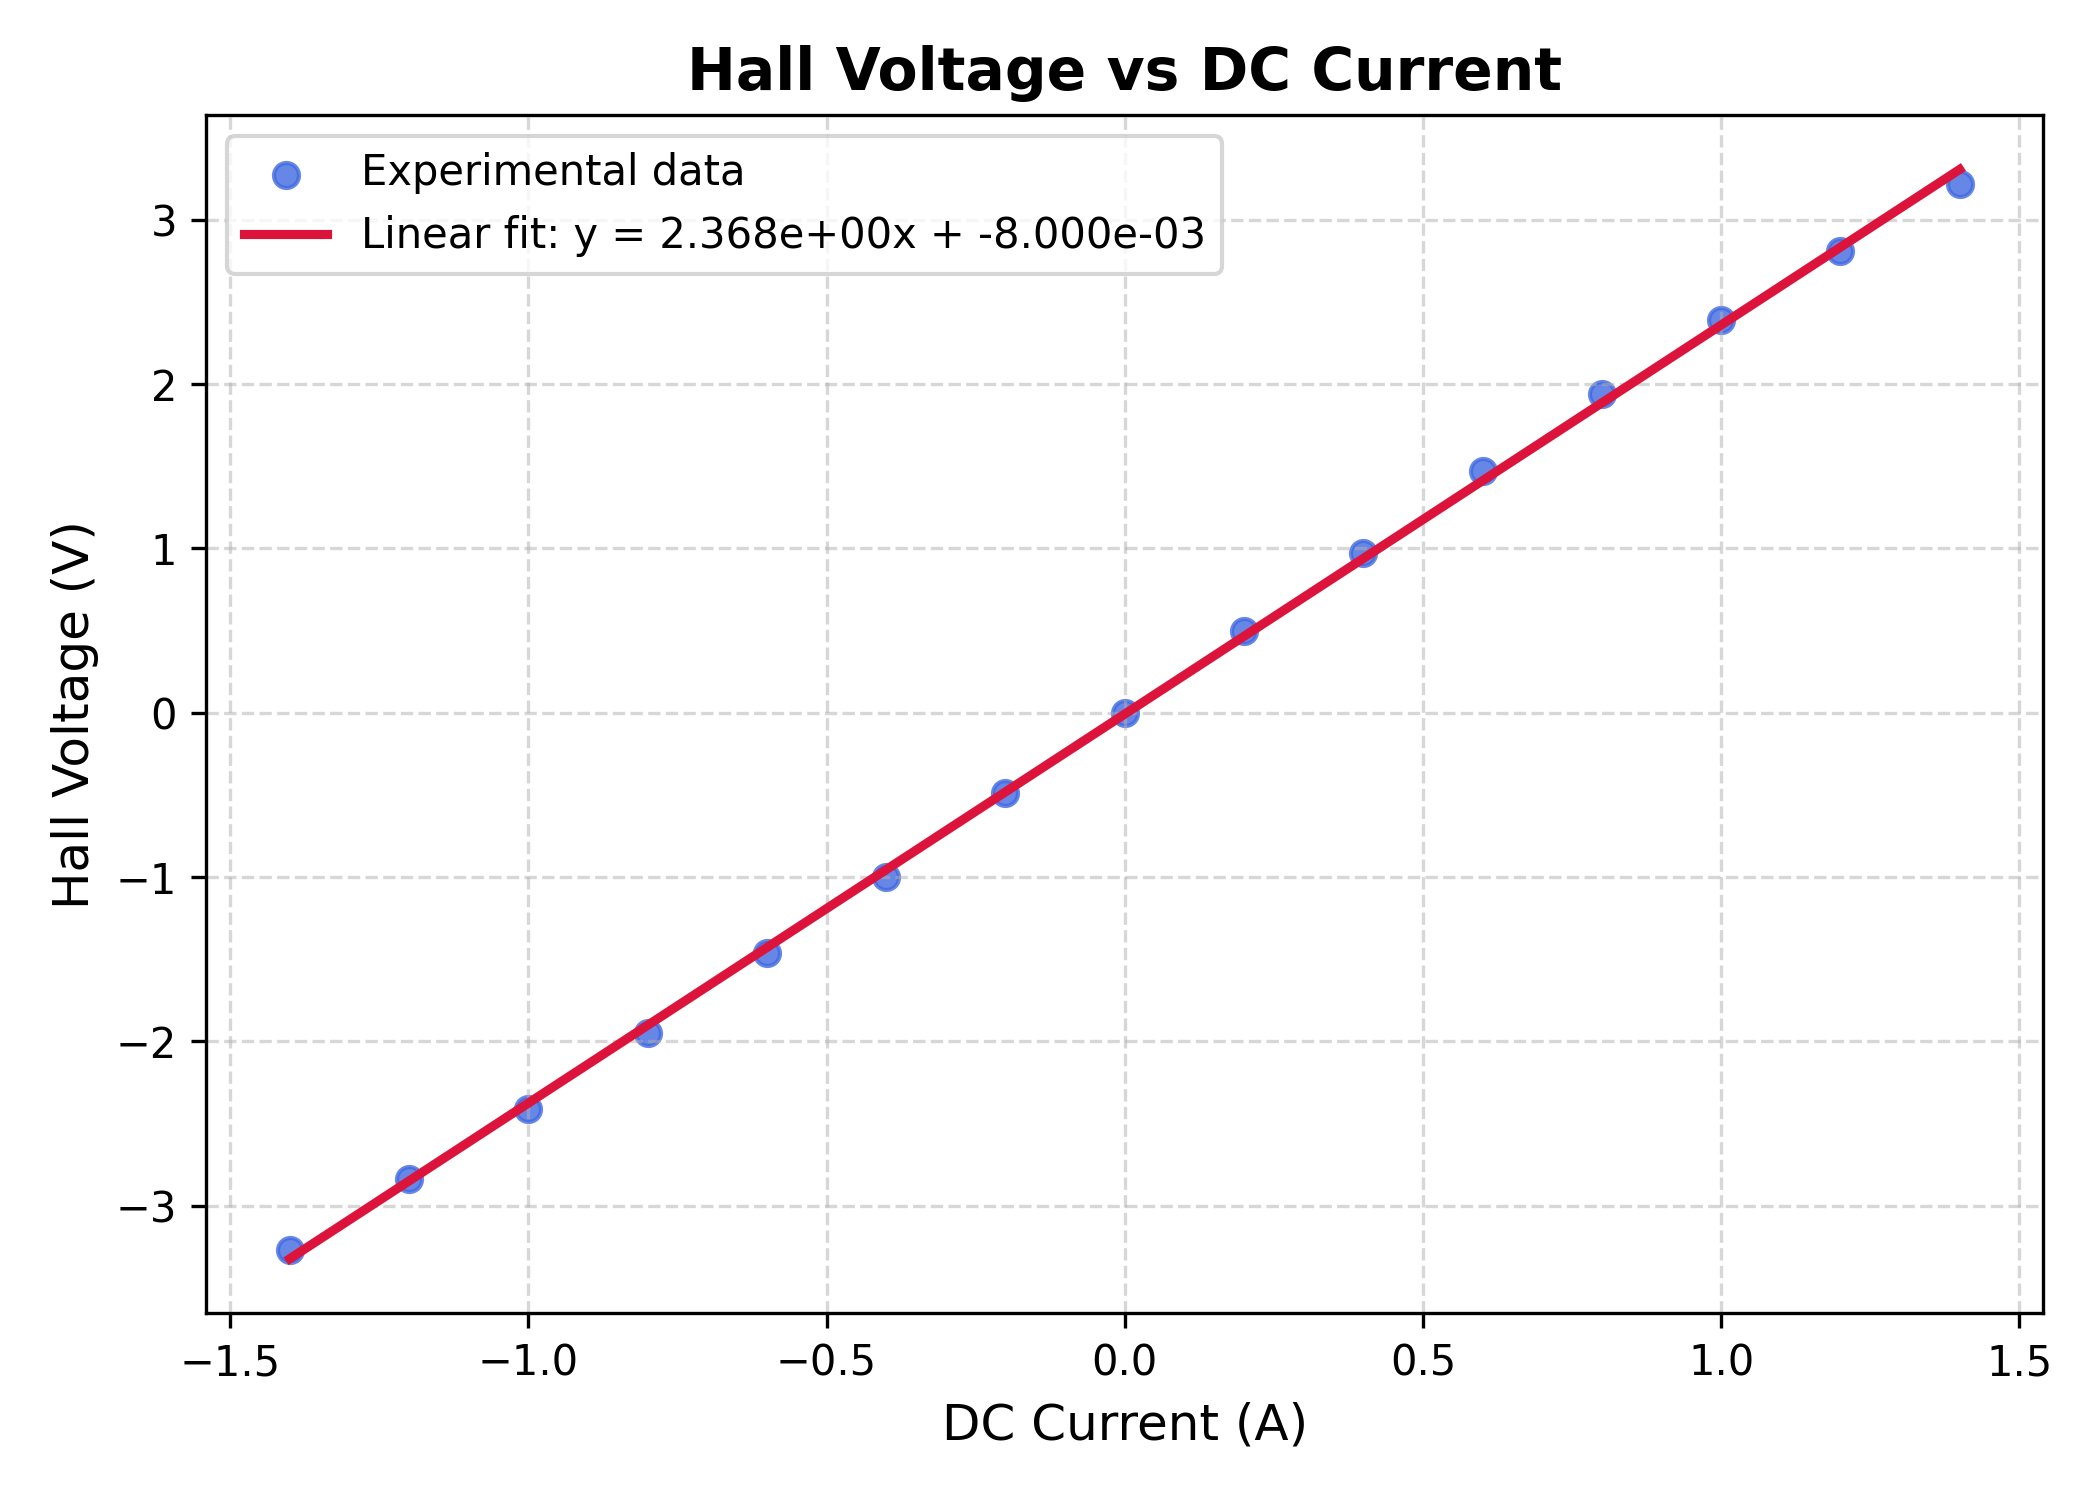
\includegraphics[width=8.5cm]{figures/hall_voltage_vs_current.png}
    \caption{Tensão versos Coerente}
    \label{fig:hall_voltage_vs_current}
\end{figure}

\hspace{1cm} A análise do gráfico demonstra que a tensão de saída varia linearmente com a corrente aplicada, indicando o comportamento linear do circuito magnético dentro da faixa de operação observada.

\hspace{1cm} Em seguida, aplicou-se a relação $B = \frac{NI}{\mathfrak{R}A} $ para determinar a densidade de fluxo magnético em função da corrente, sendo então construída a curva $B \times V$ para análise da sensibilidade do sensor.

\begin{table}[htbp]
    \centering
    \caption{Tensão de Saída e Densidade do Campo Magnético}
    \label{tab:Densidade_de_campo}
    \vspace{0.25cm}
    \begin{tabular}{ccc}
        \hline
        \rule{0pt}{3ex}\textbf{\textbf{V}}$_{saida}$ \textbf{s/ offset [V]} & \textbf{B} $\frac{Wb}{m^2}$ \\[5pt]
        \hline
        \rule{0pt}{3ex}3.22 & 0.047600 \\
        2.81 &  0.040800 \\
        2.39 &  0.034000 \\
        1.94 &  0.027200 \\
        1.47 &  0.020400 \\
        0.97 &  0.013600 \\
        0.50 &  0.006800 \\
        0.00 &  0.000000 \\
        -0.49 &  -0.006800 \\
        -1.00 &  -0.013600 \\
        -1.46 &  -0.020400 \\
        -1.95 &  -0.027200 \\
        -2.41 &  -0.034000 \\
        -2.84 &  -0.040800 \\
        -3.27 &  -0.047600 \\[5pt]
        \hline
    \end{tabular}
\end{table}

\hspace{1cm} Verifica-se que, devido à linearidade do circuito, o módulo da densidade do campo magnético é proporcional ao módulo da corrente aplicada, e que o sentido da corrente determina a direção do campo no interior do sensor Hall.

\hspace{1cm} Os resultados também evidenciam que materiais de alta permeabilidade magnética, como a ferrite, são essenciais para o bom desempenho do sensor Hall. Considerando que a permeabilidade do ar é cerca de 30 vezes menor que a da ferrite, o aumento da fração de volume ocupada por ferrite e a consequente redução da relutância total resultam em campos magnéticos mais intensos e, portanto, em tensões Hall mais precisas. Outra estratégia de aprimoramento seria o aumento do número de espiras do enrolamento, o que também ampliaria o campo gerado e a sensibilidade do sensor.

% {\Huge PLOTAR GRÁFICO}

\begin{figure}[h]
    \centering
    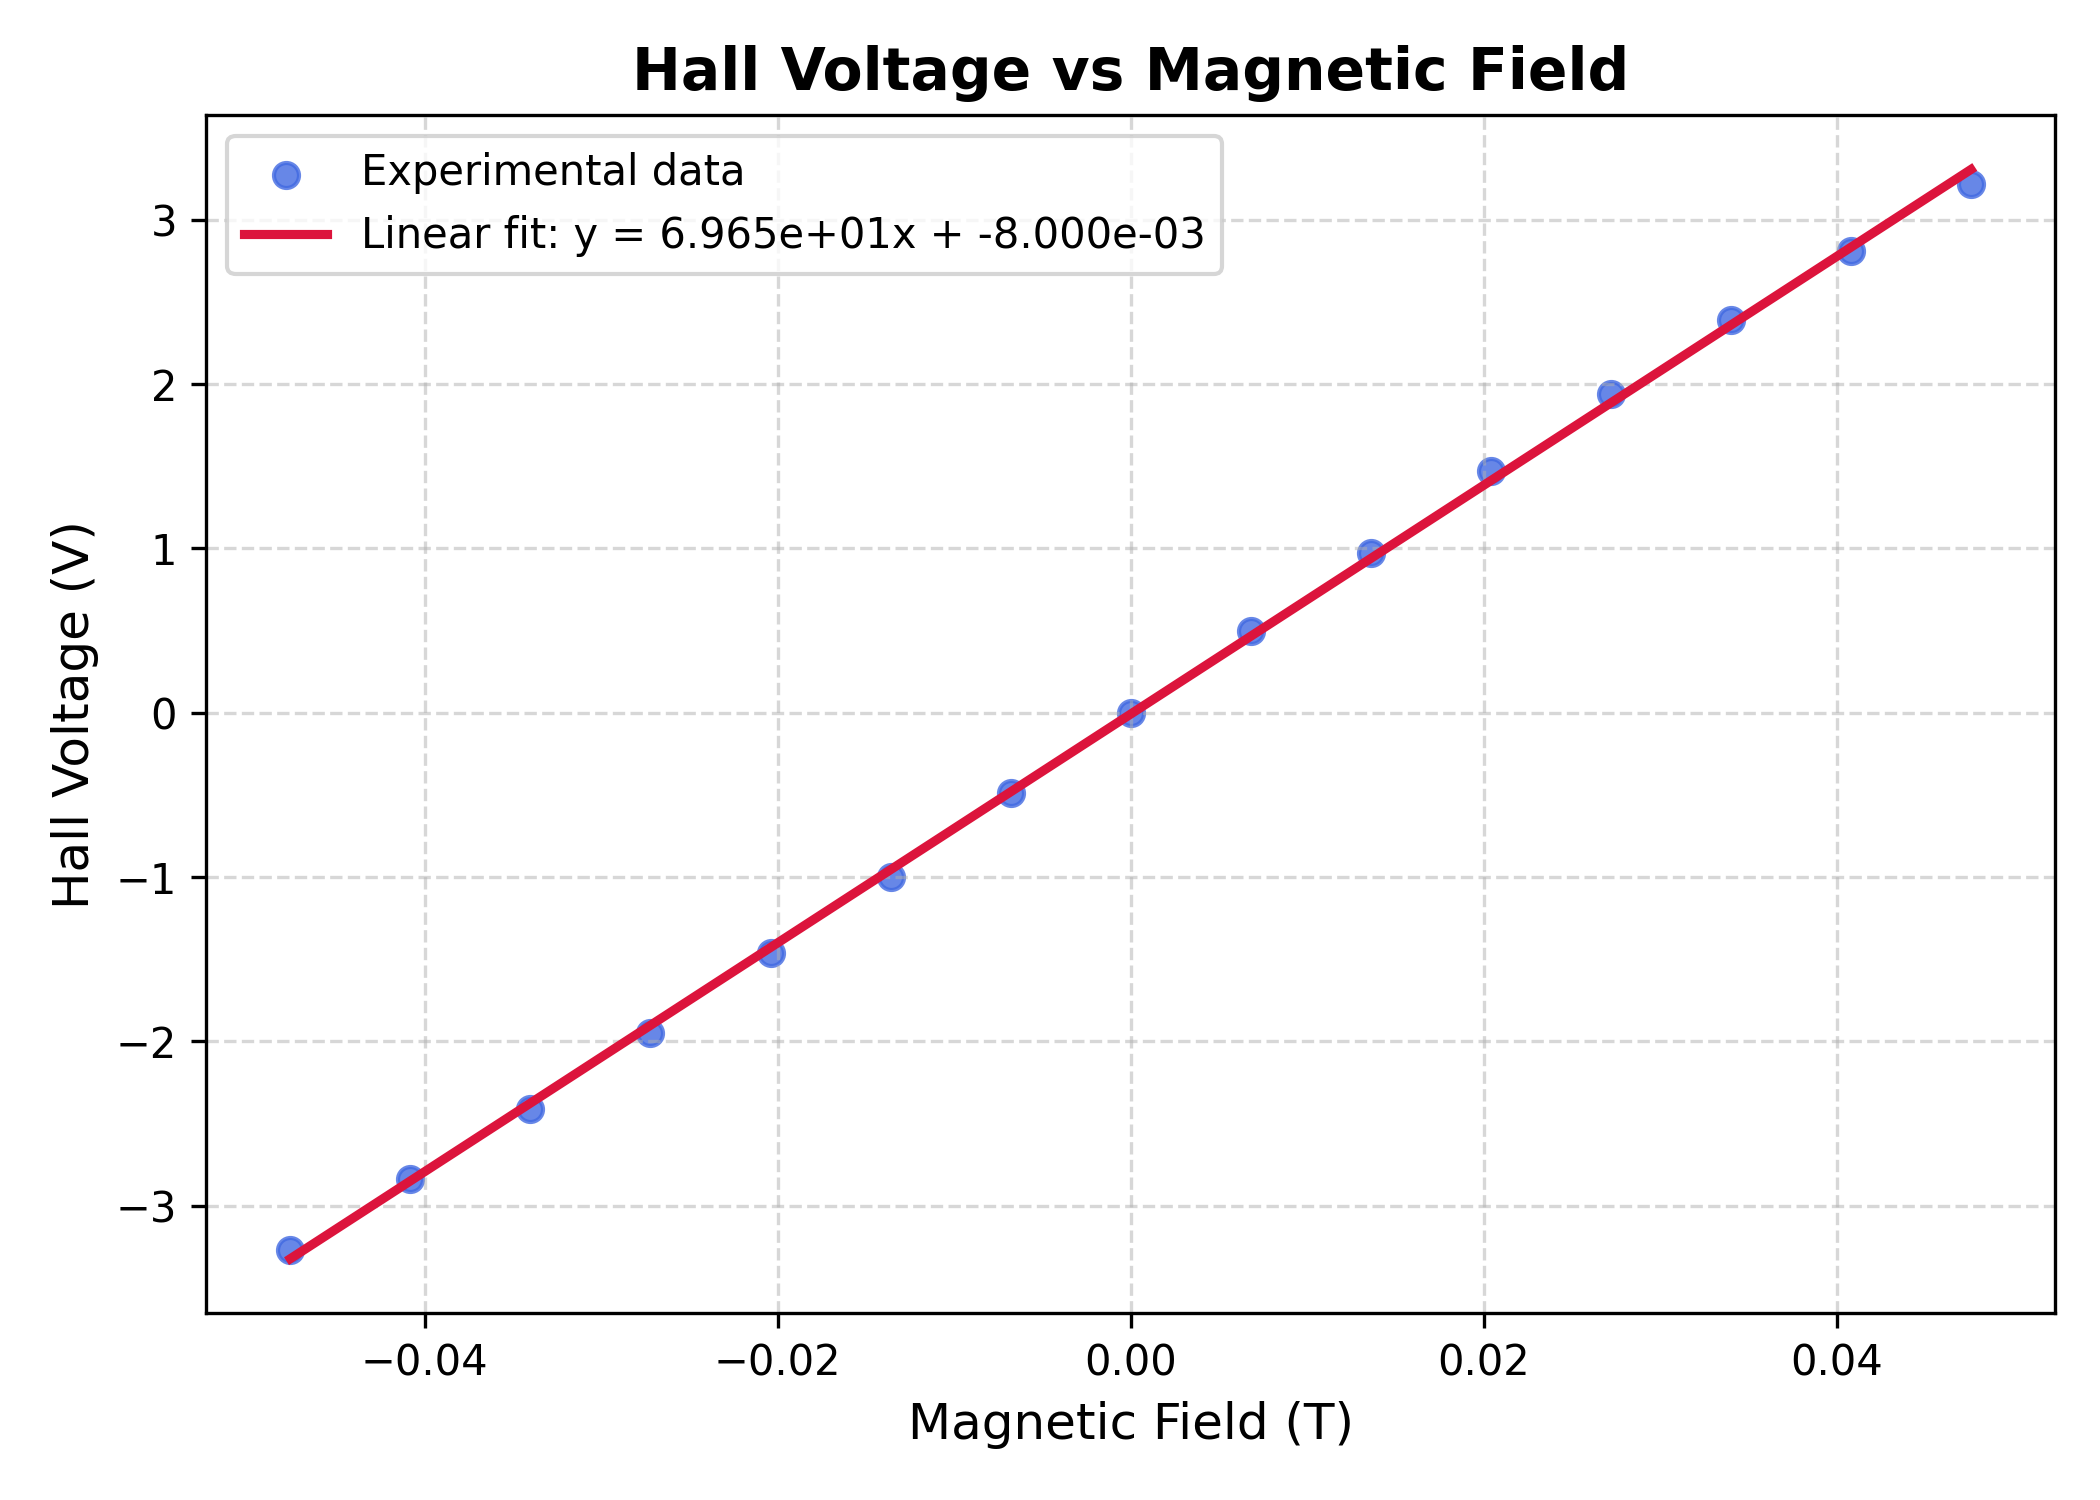
\includegraphics[width=8.5cm]{figures/hall_voltage_vs_B.png}
    \caption{Tensão vs Campo}
    \label{fig:hall_voltage_vs_B}
\end{figure}

\section{CONCLUSÃO}

\hspace{1cm} Os resultados obtidos neste experimento demonstram que a curva de resposta DC do sensor Hall está em plena concordância com o comportamento teórico esperado, validando as relações entre tensão de saída, corrente aplicada e densidade de campo magnético. Além disso, foi possível determinar e analisar a permeabilidade magnética do material de ferrite, observando sua influência direta sobre a intensidade do campo.

\hspace{1cm} Conclui-se que o efeito Hall constitui um fenômeno de grande relevância tecnológica, com ampla aplicação em sistemas de medição, controle e automação. Um exemplo clássico é o uso de sensores Hall em sistemas automotivos, especialmente para a detecção da velocidade de rotação das rodas, onde o movimento de um disco ferromagnético diante do sensor gera variações de fluxo magnético detectáveis de forma precisa e confiável.

\section{REFERENCIAS BIBLIOGRAFICAS}

\small
\begin{enumerate}

    \item CESCHIN, Artemis M. Apostila de materiais eletricos e magneticos.
    
    \item REZENDE, Sergio M. Materiais e Dispositivos Eletrônicos. 2ª ed. São Paulo: Editora Livraria da Física, 2004.

    % \item BOSCH. Speed Sensor Hall-Effect HA-Di. [online]. Disponível em: \url{https://www.bosch-motorsport.com/content/downloads/Raceparts/en-GB/53422859208177803.html#:~:text=This%20sensor%20is%20designed%20for,place%20of%20the%20sensors%20diff}

    \item HAYT, W. H. Jr. Eletromagnetismo. 6ª ed. Rio de Janeiro: LTC, 1995.
    
\end{enumerate}

\end{document}